\documentclass[12pt,spanish]{article}
\usepackage[spanish]{babel}
\usepackage{graphicx}
\usepackage{texdraw}
\usepackage{subcaption}
\usepackage{multirow}
\usepackage[hidelinks]{hyperref}
\usepackage{caption}
\usepackage{multicol}
\usepackage[outputdir=build]{minted}
\usepackage[skins,minted,breakable]{tcolorbox}
\usepackage{float}
\usepackage{array}
\graphicspath{ {../img/} {../../LaTeX/img/} {/home/csp98/latex/img/}}
\selectlanguage{spanish}
\usepackage[utf8]{inputenc}
\usepackage{graphicx}
\usepackage[a4paper,left=3cm,right=2cm,top=2.5cm,bottom=2.5cm]{geometry}
\newtheorem{ppio}{Principio }
\makeindex

\begin{document}
\begin{titlepage}

\newlength{\centeroffset}
\setlength{\centeroffset}{-0.5\oddsidemargin}
\addtolength{\centeroffset}{0.5\evensidemargin}
\thispagestyle{empty}

\noindent\hspace*{\centeroffset}
\begin{minipage}{\textwidth}

\centering
\includegraphics[width=0.9\textwidth]{logo_ugr.jpg}\\[1.4cm]

\textsc{ \Large Algorítmica\\[0.2cm]}
\textsc{GRADO EN INGENIERÍA INFORMÁTICA}\\[1cm]

{\Huge\bfseries Práctica 2\\}
\noindent\rule[-1ex]{\textwidth}{3pt}\\[3.5ex]
{\large\bfseries El elemento en su posición}
\end{minipage}

\vspace{1.5cm}
\noindent\hspace*{\centeroffset}
\begin{minipage}{\textwidth}
\centering

\textbf{Autores}\\ {María Jesús López Salmerón \\ Nazaret Román Guerrero \\ Laura Hernández Muñoz \\ José Baena Cobos  \\ Carlos Sánchez Páez}\\[2.5ex]
\includegraphics[width=0.3\textwidth]{etsiit_logo.png}\\[0.1cm]
\vspace{1.5cm}
\includegraphics[width=0.5\textwidth]{decsai.jpg}\\[0.1cm]
\vspace{1cm}
\textsc{Escuela Técnica Superior de Ingenierías Informática y de Telecomunicación}\\
\vspace{1cm}
\textsc{Curso 2017-2018}
\end{minipage}
\end{titlepage}
\tableofcontents
\thispagestyle{empty}
\listoftables
\listoffigures
\newpage
\setcounter{page}{1}
%%%%%%%%%%%%%%%%%%%%%%%%Comienzo del documento%%%%%%%%%%%%%%%%%%%%%%%%%%%%%%%
\section{Descripción de la práctica}

El objetivo de esta práctica es diseñar un algoritmo para resolver el problema del \textit{elemento en su posición}. Este algoritmo consiste en los siguiente:\\
Dado un vector $v$, determinar si $\exists i : v[i]=i $
Se implementarán dos versiones de este algoritmo: una siguiendo el algoritmo obvio y otra empleando la estrategia \emph{Divide y Vencerás}. \\

Para generar los vectores, utilizaremos el generador disponible en \textit{decsai.ugr.es}.

\section{Algoritmos diseñados}

\begin{figure}[H]
\begin{minted}[linenos]{c++}
int elementoEnSuPosicion(const vector<int> v) {
	for (int i = 0; i < v.size() ; i++)
		if (v[i] == i)
			return i;
	return -1;
}
\end{minted}
\caption{Algoritmo clásico}
\label{alg:clasico}
\end{figure}

\begin{figure}[H]
\begin{minted}[linenos]{c++}
int elementoEnSuPosicion(const vector<int> v, const int ini, const int fin) {
	if (ini == fin) {	//Caso base, vector de un solo elemento
		if (v[ini] == ini)
			return ini;
		else
			return -1;
	}
	else {	//Partimos en dos el vector y llamamos recursivamente
		int mitad = (ini + fin) / 2;
		int pos_izq = elementoEnSuPosicion(v, ini, mitad);
		int pos_dcha = elementoEnSuPosicion(v, mitad + 1, fin);
		if (pos_izq != -1)
			return pos_izq;
		else
			return pos_dcha;
	}
}	
\end{minted}
\caption{Algoritmo Divide y Vencerás}
\label{alg:dyv}
\end{figure}

\newpage

\section{Estudio de eficiencia}

En esta sección procederemos a estudiar la eficiencia de los algoritmos en cuestión.

\subsection{Eficiencia teórica}

Como podemos ver en \textcolor{blue!60}{\hyperref[alg:clasico]{el algoritmo clásico}}, iteramos por el bucle hasta encontrar un elemento en el que se cumpla la condición ($v[i]=i$). Por tanto, en el peor de los casos recorreremos el bucle completo, siendo la eficiencia de \textbf{O(n)}.\\

En cuanto al \textcolor{blue!60}{\hyperref[alg:clasico]{algoritmo Divide y Vencerás}}, nuestro algoritmo es recursivo y la metodología es la siguiente:
\begin{itemize}
	\item \textbf{Caso base}. El vector consta de un solo elemento.
	\item Calculamos la posición del elemento mitad del vector.
	\item Llamamos recursivamente a la función desde el tamaño inicial hasta la mitad y desde la mitad + 1 hasta el final.
	\item Comprobamos si el elemento se encuentra en la mitad izquierda. En caso afirmativo, devolvemos \textcolor{blue!90}{su posición}.
	\item En caso contrario, devolvemos \textcolor{blue!90}{el resultado de aplicar el algoritmo en la mitad derecha}.
\end{itemize}

Como podemos ver, aun así en el peor de los casos tendremos que recorrer el vector en su totalidad, por lo que la eficiencia del algoritmo empleando la estrategia \textit{Divide y Vencerás} es \textbf{O(n)}.\\

Por tanto, podemos adelantar que debido a los costes físicos de la recursión el algoritmo \emph{clásico} será mejor que el \emph{Divide y Vencerás}.

\subsection{Eficiencia empírica}

Haciendo uso de \textcolor{blue!60}{\hyperref[sec:scripts]{los scripts diseñados}}, ejecutamos los algoritmos con los siguientes tamaños:

\begin{table}[H]
\centering
\begin{tabular}{|c|c|c|c|}
\hline
\textbf{Algoritmo}  & \textbf{Tamaño inicial} & \textbf{Tamaño final} & \textbf{Incremento}\\
\hline
Clásico & 1.000.000 & 1.480.000 & 20.000 \\
Divide y Vencerás & 1.000 & 3.400 & 100\\
\hline
\end{tabular}
\caption{Parámetros de ejecución de cada programa}
\end{table}

\begin{figure}[H]
\centering

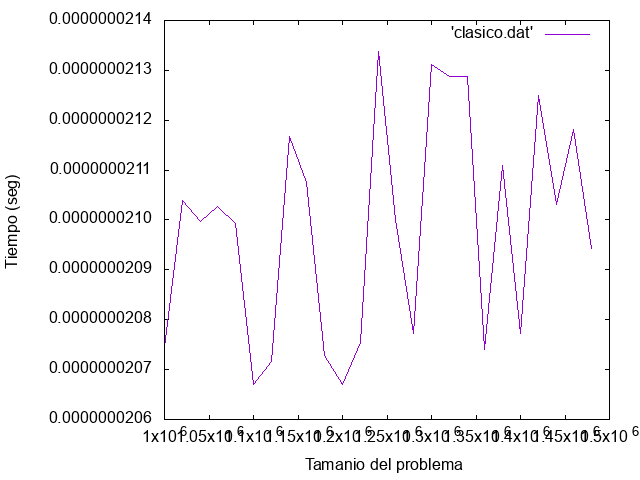
\includegraphics[scale=0.75]{clasico.png}
\vskip 0.5cm

\begin{tabular}{|c|c|}
\hline
\textbf{Tamaño} & \textbf{Tiempo (s)} \\
\hline
1000000 & 0.000819706\\
\hline
1020000 & 0.000842275\\
\hline
1040000 & 0.00085518\\
\hline
1060000 & 0.000869587\\
\hline
1080000 & 0.000885716\\
\hline
1100000 & 0.000899005\\
\hline
1120000 & 0.000922726\\
\hline
1140000 & 0.000934545\\
\hline
1160000 & 0.000951469\\
\hline
1180000 & 0.00096667\\
\hline
1200000 & 0.000988998\\
\hline
1220000 & 0.000997361\\
\hline
1240000 & 0.00101367\\
\hline
1260000 & 0.0010278\\
\hline
1280000 & 0.00104895\\
\hline
1300000 & 0.00106148\\
\hline
1320000 & 0.00108836\\
\hline
1340000 & 0.00110376\\
\hline
1360000 & 0.00113126\\
\hline
1380000 & 0.00110421\\
\hline
1400000 & 0.00114935\\
\hline
1420000 & 0.00116467\\
\hline
1440000 & 0.0011756\\
\hline
1460000 & 0.00118976\\
\hline
1480000 & 0.00121112\\
\hline

\end{tabular}


\caption{Algoritmo clásico}
\end{figure}


\begin{figure}[H]
\centering

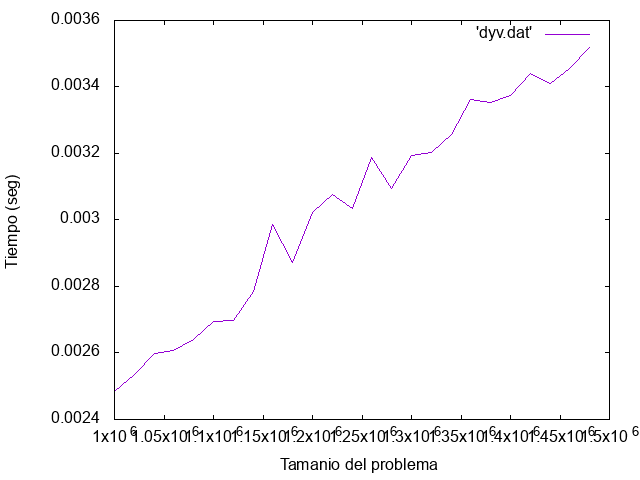
\includegraphics[scale=0.75]{dyv.png}

\vskip 0.5cm

\begin{tabular}{|c|c|}
\hline
\textbf{Tamaño} & \textbf{Tiempo (s)} \\
\hline
1000 & 0.000551096 \\
\hline
1100 & 0.000600369 \\
\hline
1200 & 0.000736414 \\
\hline
1300 & 0.000889537 \\
\hline
1400 & 0.00100999 \\
\hline
1500 & 0.00113876 \\
\hline
1600 & 0.00129452 \\
\hline
1700 & 0.00150525 \\
\hline
1800 & 0.00165492 \\
\hline
1900 & 0.00180961 \\
\hline
2000 & 0.00215437 \\
\hline
2100 & 0.00233609 \\
\hline
2200 & 0.00252987 \\
\hline
2300 & 0.00276466 \\
\hline
2400 & 0.00294883 \\
\hline
2500 & 0.00332321 \\
\hline
2600 & 0.00349556 \\
\hline
2700 & 0.00382512 \\
\hline
2800 & 0.00405147 \\
\hline
2900 & 0.00431329 \\
\hline
3000 & 0.00460976 \\
\hline
3100 & 0.00493946 \\
\hline
3200 & 0.00534553 \\
\hline
3300 & 0.00548893 \\
\hline
3400 & 0.00605759 \\

\hline
\end{tabular}


\caption{Algoritmo Divide y Vencerás}
\end{figure}

\begin{figure}[H]
\centering
\begin{tabular}{|c|c|}
\hline
\textbf{Algoritmo clásico} & \textbf{Algoritmo Divide y Vencerás} \\
\hline
0,001009366976743 & 0,002223563169903 \\
\hline
\end{tabular}
\caption{Tiempo medio (s)}
\end{figure}

\subsection{Eficiencia híbrida}

En esta sección ajustaremos los datos obtenidos a las expresiones teóricas obtenidas mediante una regresión con el objetivo de obtener su constante oculta.

\begin{figure}[H]
\centering
\begin{tabular}{|c|c|c|c|}
\hline
\textbf{Algoritmo} & \textbf{Eficiencia teórica} & \textbf{Valor de la constante oculta} & \textbf{Error} \\
\hline
Clásico & O($n$) & 8.19304e-10 &0.1441\% \\
Divide y Vencerás & O($n^2$) & 5.17311e-10 & 0.3221\% \\
\hline
\end{tabular}
\end{figure}

\newpage 

\begin{figure}[H]
\centering
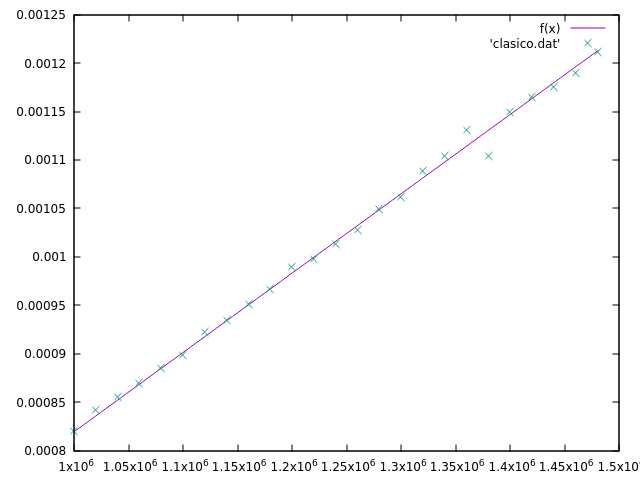
\includegraphics[scale=0.75]{hibrida_clasico.png}
\caption{Eficiencia híbrida del algoritmo clásico}
\end{figure}

\begin{figure}[H]
\centering
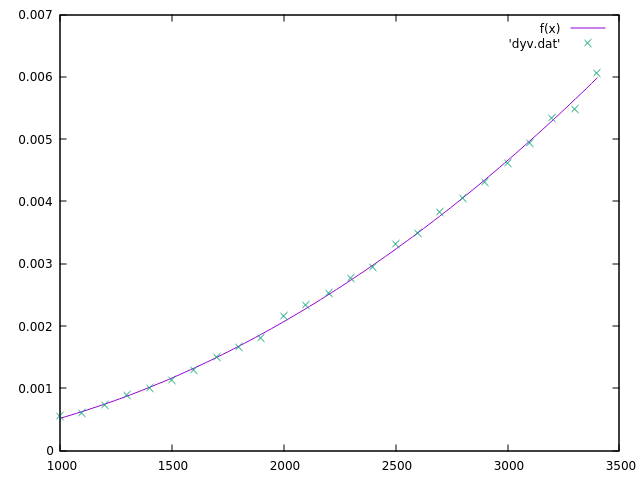
\includegraphics[scale=0.75]{hibrida_dyv.png}
\caption{Eficiencia híbrida del algoritmo Divide y Vencerás}
\end{figure}


\section{Conclusiones}


\section{Anexo: scripts implementados}
\label{sec:scripts}

\begin{figure}[H]
\begin{minted}[linenos]{bash}
#!/bin/bash
if [ $# -eq 3 ]
then
i="0"
tam=$2
#Primer argumento: programa a ejecutar
#Segundo argumento: tamaño inicial
#Tercer argumento : incremento
while [ $i -lt 25 ]
do
	./$1 $tam >> ./$1.dat
	i=$[$i+1]
	tam=$[$tam+$3]
done
else
echo "Error de argumentos"
fi

\end{minted}
%$
\caption{Script individual}
\end{figure}



\begin{figure}[H]
\begin{minted}[linenos]{bash}
#!/usr/bin/gnuplot

set xlabel "Tamanio del problema"
set ylabel "Tiempo (seg)"
set terminal png size 640,480
set output 'clasico.png'
plot 'clasico.dat' with lines
set output 'dyv.png'
plot 'dyv.dat' with lines
\end{minted}
\caption{Script de gnuplot}
\end{figure}


\begin{figure}[H]
\begin{minted}[linenos]{bash}
#!/bin/bash
	echo "Compilando..."
	g++ -o clasico clasico.cpp -O3 &&
	g++ -o dyv dyv.cpp -O3 &&
	rm -f ./clasico.dat ;
	rm -f ./dyv.dat ;
	echo "Ejecutando algoritmo clásico..." ;
	./individual.sh clasico 1000000 20000;
	echo "Ejecutando algoritmo DyV..." ;
	./individual.sh dyv 1000 100;
	echo "Generando gráficas..." ;
	./gnuplot.sh ;
\end{minted}
\caption{Script conjunto}
\end{figure}


%%%%%%%%%%%%%%%%%%%%%%%%%%%%Fin del documento%%%%%%%%%%%%%%%%%%%%%%%%%%%%%%%%
\end{document}
